\subsection{P1}


Let's consider the following conjecture. 

\begin{conjecture}[P1]
Let $a\in \cat{C}$.
A sheaf module $\sheaf{F}$ on $\rsite{C}{T}{O}/a$ is quasi-coherent \iff $\sheaf{F}$ is quasi-coherent on $\rsite{C}{T}{O}/b$ for any affine $b\rightarrow a$
\end{conjecture}

\begin{remark}\label[remark]{563}
The only if direction always holds.
\end{remark}



\begin{lemma}[P1 holds with enough affines]\label[lemma]{569}
P1 holds for any ringed site with enough affines.
\end{lemma}

\begin{proof}
Quasi-coherence is a local property. So if every object admits a affine cover P1 holds.
\end{proof}

\begin{lemma}[Finite poset has enough affines]\label[lemma]{571}
Any finite poset has enough affines.
\end{lemma}

\begin{proof}[NA-chain proof]
Let $x_0\in C$. 
If $x_0$ is covered by the maximal sieve only or the maximal sieve and the empty sieve, it is affine and we are done. 
Assume otherwise.
Let $S = \{y_i \rightarrow x_0\}$ be a non-maximal, non-empty cover of $x_0$.
Then $S$ does not contain isomorphisms.

We can associate to any non-maximal non-empty covering sieve $S$ of an element $x_0$,
the set of all NA-chains $x_0\leftarrow x_1 \leftarrow \ldots \leftarrow x_n$.
An NA-chain, associated to $R$, is a chain of maps ending in $x_0$ such that $x_i \leftarrow x_{i+1}$ is contained in a non-maximal, 
non-empty cover of $x_i$, where $x_0\leftarrow x_1$ is contained in $R$.

By finiteness of $C$, any chain of maps is bounded by the size of $C$ or contains a cycle. 
If a chain contains a cycle, it contains isomorphisms. 
By construction, no isomorphism can be present in a NA-chain. 
Therefore the length of any NA-chain is bounded by $\card{C}$.

Let $H$ be a NA-chain associated to $S$ of maximal length $m$. 
Then the last map $\ldots \leftarrow h \leftarrow g$ in $H$ has an affine object $g$ as domain,
because $H$ cannot be increased and so $g$ has no non-maximal, non-empty coverings which makes it affine.
Also the non-maximal, non-empty covering of $h$ where this map appears must be an affine covering by applying the same reasoning to the other objects occurring in it. 
Hence all objects occurring at the $(m-1)$th place in any NA-chain admits an affine cover.
Let $i\leq m-1$. Assume all elements at the $(i-1)$th place admit an affine cover. 
Let $b$ be a object occurring at the $(i-1)$th place in a chain. It is either affine or all objects in any non-maximal, non-empty cover occur at the $i$th place in some chain hence admit an affine cover. Therefore any non maximal, non empty cover on $b$ can be refined to an affine cover. This provides us with an affine cover of $b$.
By reversed induction, $x_0$ admits a affine cover.
\end{proof}

\begin{lemma}[Non-quasi-coherent sheaf]\label[lemma]{579}
Any category admits a non-quasi-coherent sheaf.
\end{lemma}

\begin{proof}
%TODO: nakijken
\begin{example}\label[example]{50c}
Let $C$ be a ringed site with no affines. 
Therefore no object can have the empty sieve as a covering sieve, because that would make all sheafs trivial restricted at this object.
Let $\sheaf{O}$ be its structure sheaf.

Let $a$ be an object of $C$.
Let $b$ be an object of $C$ such that $\Hom{b}{a}=\emptyset$.

The following situation, the commuting square with conditions on the maps and objects, will be called $S1$.
Note that $a,b$ are fixed and not variables in $S1$. 

%TODO: improve this diagram
\begin{center}
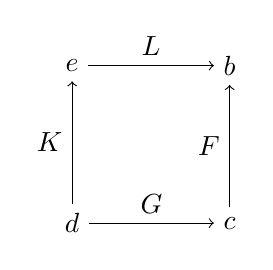
\begin{tikzpicture}[node distance=2cm, auto]
  \node (C) {$c$};
  \node (B) [above of =C] {$b$};
  \node (D) [left of =C] {$d$};
  \node (E) [above of =D] {$e$};
  \draw[->] (C) to node {$F$} (B);
  \draw[->] (D) to node {$G$} (C);
  \draw[->] (D) to node {$K$} (E);
  \draw[->] (E) to node {$L$} (B);
\end{tikzpicture}
\end{center}

With $\sheaf{O}(d)\neq 0$, $\Hom{e}{a}=\emptyset$ and $\Hom{c}{a}\neq\emptyset$ .

Assume that for any $S$ a covering sieve on $b$.

1) every map $F\in S$ as in $S1$, so $F$ has codomain $b$ and its domain maps to $a$,
we can find maps $G,K,L$ to complete to $S1$ with $L\in S$.

2) For every $L\in S$ as in $S1$, so $L$ has codomain $b$ and its domain does not map to $a$, we can complete the to get $S1$.

Consequences: Every non-empty covering sieve of $b$ contains maps $L$ and $F$ that fit in $S1$.
'Objects under $a$ get under every object under $b$'.
Call this assumption $A1$ en $A2$.

Define the presheaf $\presheaf{F}$ as

\[ x \mapsto \sheaf{O}(x) \mbox{ if } \Hom{x}{a}=\emptyset, \]
\[ x \mapsto \sheaf{O}(x)[y] \otherwise,\] 

\[ u \xrightarrow{f} v \mapsto \sheaf{O}(f) \mbox{ if } \Hom{u}{a} = \emptyset, \]
\[ u \xrightarrow{f} v \mapsto (\sheaf{O}(u) \rightarrow \sheaf{O}(u)[y]) \circ \sheaf{O}(f) 
\mbox{ if } \Hom{u}{a} \neq \emptyset \; \& \; \Hom{v}{a} = \emptyset,\]
\[ u \xrightarrow{f} v \mapsto \sheaf{O}(f) \otherwise.\]

Let $G = \presheaf{F}^{++}$.


%%show G(b) = \sheaf{O}(b)

Let $S$ be a covering sieve on $b$. If $S$ is empty, then $G(b) = 0 = \sheaf{O}(b)$.
Assume otherwise.
Let $(x_f)$ be a matching family indexed by $S$.
Let $x_f\in G(u)\setminus O(u)$ for $u\xrightarrow{f} b$ such that $\Hom{u}{a} \neq \emptyset$, 
which is possible by $A2$. Set $F=f$ and complete to $S1$. Then $\presheaf{F}(G)(x_F)= \presheaf{F}(K)(x_L) = x_{KL}$ since it is a matching family,
which is impossible because $\presheaf{F}(G)(x_F)$ is not in the image of $\presheaf{F}(K)$.
So all matching families $(x_f)$ have components that are elements of $O(\Dom{f})\subset G(\Dom{f})$, 
which already have unique amalgamations in $\sheaf{O}(b)$. 
Hence $G(b)= \sheaf{O}(b)$.

%%Show G is not quasi-coherent
Let $U$ be a global cover of the category.
By A1, $U(b)$ contains an element $g:e\rightarrow b$ with $\Hom{e}{a} = \emptyset$.
Set $g=L$ and complete $S1$.
The element $y\in G(d)$ is not generated locally by sections of $G(e)$.
Hence $G$ is not locally presentable.

\emph{Examples that satisfy A1\&A2}
\begin{itemize}
\item Open category of any irreducible space.
\item Neighbourhood space of any point in any topological space.
\item categories with pullbacks, terminal object and are irreducible.
\end{itemize}
\end{example}
\end{proof}

\begin{example}[Stacks 01BL example]\label[example]{581}
%Setting
Let $L = (\R, O_R)$ be the real line with the euclidean topology and the sheaf of continuous real valued functions as structure sheaf.
Let \[X = \frac{\bigcup_{i=0}^\infty L_i}{\sim}\] with $[i,x] \sim [j,y]$ \iff $i=j$ and $x=y$ or $y=x=0$. 
The real lines are glued to each other at zero.
Define the open $U_n\subset X$ as $U_n\cap L_i=(-\frac{1}{n},\frac{1}{n})$. 
These opens form a basis of neighbourhoods of $0$.
Let $f:\R\rightarrow \R$ be any continuous function such that $f(x)=0$ 
if $x\in (-1,1)$ and $f(x)=1$ if $x\in (-\infty,-2)\cup (2,\infty)$.
Let $f_n(x)=f(nx)$.

%Define map
Define the sheaf map 
\[\coproduct_i O_R \xrightarrow{\alpha} \coproduct_{ij} O_R,\]
\[e_i \mapsto \sum_{j} f_i \indicator_{L_j} e_{ij}.\]

To proof that this is well-defined, we need to show that the sum $\sum_{j} f_i \indicator_{L_j} e_{ij}$ 
is locally finite for every $i$.
Let $[k,y]\in X$. If $y\neq 0$, then \[W_{[k,y]}=\{[k,z]\in X \mid z\in(y-\delta, y+\delta\}\subset L_k\] is open in $X$
and $\alpha_{W_{[k,y]}}(e_i)  = f_ie_{ik}$ for any $\delta< \abs{\frac{y}{2}}$.
If $y=0$, then $\alpha_{U_n}(e_i) = 0$ if $n>i$ because $f_i$ is zero on $U_n$.
Hence we found a cover on which our sum is locally finite, which makes $\alpha$ well-defined.


%Tilde and restriction commute
Let $U$ be any open of any topological space $X$. 
Let $\presheaf{F}$ be any presheaf.
Consider the map of presheafs
\[\restr{\presheaf{F}}{U}^{+}\xrightarrow{g} \restr{\presheaf{F}^{+}}{U}\]

defined by the components

\[g_V: \colim{S\in \cov(V)} \match{S}{F} \xrightarrow{\mbox{id}} \colim{S\in \cov(V)} \match{S}{F}.\]

Every component is a isomorphism, hence $g$ is an isomorphism.

%Domain&codomain are associated sheafs
The adjunction $(\Lambda(-),\Gamma(X,-))$ implies that $\Lambda(-)$ commutes with arbitrary colimits.
Moreover
\[O_X \iso \Lambda(\Gamma(X,O_X))\]

so

\[\coproduct_i O_R \iso \Lambda(\coproduct_i \Gamma(X,O_X)).\]

This shows that $\alpha$ is a morphism between associated sheafs.
Let $\beta: \coproduct_i \Gamma(U,O_X)\rightarrow \coproduct_{ij} \Gamma(U,O_X)$ for some open $U$.
Then $\Lambda(\beta)(e_i) = \sum_{j\in J_i} a_{ij} e_{ij}$ where $J_i$ is finite for every $i$.

%Contradiction
Assume that $\alpha = \Lambda(\beta)$ over some neighbourhood $U$ of $0$.
Then there exists a $m$ such that $U_m\subset U$. Let $k>2m$.
Then $f_k\neq 0$ on $U_m$, hence $f_k \indicator_{L_j}\neq 0$ on $U_m$ for every $j$ and so no co{\"e}fficients vanish of $\alpha_{U_m}(e_k) =\sum_{j} f_k \indicator_{L_j} e_{kj}$. 
This contradicts $\alpha=\Lambda(\beta)$.

\end{example}

\begin{example}[Category without enough affines \#1]\label[example]{585}
%%% Example moved to N(y) setting
Let $X,f_j$ and $U_n$ be as in the previous example.
Define the full subcategory $N(y)\xrightarrow{i}\opens(X)$ of all opens $U$ that contain the point $y\in X$.

This category has all fibre products. Let $U\rightarrow V \leftarrow W$ be two morphisms.
Then $U \leftarrow U\cap W \rightarrow W$ is the pullback.

On this category $N(y)$, let a family $\{f_i:U_i\rightarrow U\}$ be covering if $\union_i f_i(U_i) = U$. 

Let $V\xrightarrow{f} U$ be an isomorphism, then $f(V)=U$ so $\{f\}$ is a covering family.

Let $\{U_i \xrightarrow{f_i} U\}$ be a covering family. 
For every $i$, let $\{U_{ij}\xrightarrow{f_{ij}} U_i\}$ be a covering family. 
By definition this gives that $\union_i f_i(U_i)=U$ and $\union_j f_{ij}(U_ij)=U_i$ for every $i$. 
Hence \[\union_{i,j} (f_i \circ f_{ij}) (U_{ij}) = \union_{i} f_i(U_i)=U\] and so the family 
$\{U_{ij}\xrightarrow{f_i \circ f_{ij}} U\}$ is covering.

Let $V\rightarrow U$ be a morphism in $N(y)$ and $\{U_i \xrightarrow{f_i} U\}$ be a covering family on $U$.
This tells us that $\union_i f_i(U_i)=U$, hence also $\union_i g_i(U_i\cap V) = V$ where $g_i:U_i\cap V\rightarrow V$ is the pullback of $f_i$. 
Hence $\{U_i\cap V\xrightarrow{g_i}V\}$ is a covering family of $V$.

All criteria for a pretopology are established. Let $\tau$ be the generated Grothendieck topology.

%%i is continuous
Let $\sheaf{F}$ be a sheaf on $\opens{X}$.
Let $\hat{\sheaf{F}} = \sheaf{F}\circ i$.
Let $\cover{U_i}{V}$ be a covering family on $V$ in $N(y)$.
Let $(x)_i$ be a matching family of $\hat{\sheaf{F}}$ indexed by $\cover{U_i}{V}$, so $x_i \in \hat{\sheaf{F}}(U_i) = \sheaf{F}(U_i)$.
Note that $\cover{U_i}{V}$ is also a covering family on $V$ in $\opens{X}$, hence $(x)_i$ is also a matching family of $\sheaf{F}$ on $V$.
Since $\sheaf{F}$ is a sheaf, there exists a unique amalgamation $x\in \sheaf{F}(V)=\hat{\sheaf{F}}(V)$ such that $x=x_i$ in $\sheaf{F}(U_i)=\hat{\sheaf{F}}(U_i)$. 
This shows that $\hat{\sheaf{F}}$ is a sheaf, hence $i$ is continuous.

Let $\sheaf{O}_{X,y} = \sheaf{O}_X\circ \tau$. This is a sheaf of rings by the previous.
We constructed a ringed site $(N(y),\tau,\sheaf{O}_{X,y})$.

%%adjunctions
Let $F$ be the inclusion functor from the category of sheafs to the category of presheafs. 
We have the adjunctions:

\begin{enumerate}
\item $(\Lambda(-),\Gamma(X,-))$,
\item $((-)^{++},F)$.
\end{enumerate}

%%coproduct is still associated, holds in every ringed site
The structure sheaf $O_{X,y}$ is, trivially, isomorphic to $\Lambda(\Gamma(X,O_{X,y}))$.
By adjunction (2)
\[\coproduct_i \sheaf{O}_{X,y} \iso (\coproduct_i \sheaf{O}_{X,y})^{+s},\]
where the coproduct on the left hand side is in the category of sheafs and the coproduct on the right hand side in the category of presheafs.

By adjunction (1)
\[\coproduct_i \Lambda(\Gamma(X,O_{X,y})) \iso \Lambda(\coproduct_i \Gamma(X,O_{X,y})).\]

Combine these 3 observation to get

\[\coproduct_i \sheaf{O}_{X,y} \iso \Lambda(\coproduct_i \Gamma(X,O_{X,y})),\]

which shows that $\coproduct_i \sheaf{O}_{X,y}$ is quasi-coherent.


%%Define \alpha
Set $y=0\in X$.
Define the sheaf map 
\[\coproduct_i O_{X_y} \xrightarrow{\alpha} \coproduct_{ij} O_{X_y},\]
\[e_i \mapsto \sum_{j} f_i \indicator_{L_j} e_{ij}.\]

%%Proof \alpha is well-defined
Fix $i$. We will prove that $\alpha_X(e_i)$ is a well-defined global section.
Let $m>i$. Let $V_k=L_k\cup U_m$ and $\cover{V}=\{V_k\}$.
By construction $f_i$ is zero on $U_m$, hence $f_i \indicator_{L_j}$ is zero on $V_k$ if $k\neq j$ and so $\sum_{j} f_i \indicator_{L_j} e_{ij} = f_i\indicator{L_k}e_{ik}$ on $V_k$.
This shows that $\alpha_X(e_i)$ is a well-defined section on any element of the cover $\cover{U_i}{V}$ and
this family is matching since the sections are functions and the 'restriction' maps are actual restriction.

%%Absence of a \beta for every element
Assume there exists $\beta: \coproduct_i \Gamma(V,O_{X,y}) \rightarrow \coproduct_{ij} \Gamma(V,O_{X,y})$ such that $\Lambda(\beta)=\alpha_V$.
Then $\alpha_V(e_i)=\sum_{j} f_i \indicator_{L_j} e_{ij}$ is not just locally finite over some cover, but actually finite globally on $V$ for all $i$.
So almost all $f_i \indicator_{L_j}$ are zero on $V$. 
Note that $y\in V$, so $U_d\subset V$ for some $d$. 
Let $i>2d$, then $f_i\neq 0$ on $(-\frac{1}{d},\frac{1}{d})$ and so $f_i \indicator_{L_j}\neq 0$ on $U_d$ for any $j$.
Hence $\alpha_V(e_i)=\sum_{j} f_i \indicator_{L_j} e_{ij}$ is not a finite sum for $i>2d$. 
This contradicts our assumption.

%%Mistake
Let $U\subset X$ be $U\cap L_j = U_{j}$. Fix $i$.
Then $f_i\indicator_{L_j}=0$ if $i<j$, hence \[\sum_{j} f_i \indicator_{L_j} e_{ij}=\sum_{j\leq i} f_i \indicator_{L_j} e_{ij}\] is a finite sum.

%%Conclude no element is affine
The restriction of any quasi-coherent sheaf is quasi-coherent. 
Observe that $\alpha$, and its restrictions, is a morphism between quasi-coherent sheafs but does not come from a map of modules.
Therefore $\Lambda(-)_V: \Gamma(V, O_{X,y})-\mbox{Mod} \rightarrow \qcoh{V}$ is not full for any $V$ and no object $V$ is affine in $N(y)$.
\end{example}

\begin{example}[Category without enough affines \#1]\label[example]{589}
%TODO
\end{example}

\begin{example}[General P1 does not hold]\label[example]{58d}
The category $C$ is $\Z \times \Z$ with the usual ordering.
An element $(i,j)$ is only non-trivially covered by $\{(i,j-1)\rightarrow (i,j),(i-1,j)\rightarrow (i,j)\}$.
Let $k$ be any field.
Let $R = k[x_{ij}| i,j\in \Z]$. 
Define the structure sheaf as $O(i,j) = R[x_{kl}^{-1}| i\leq k \; \& \; j \leq l]$.

Fix $(a,b)\in C$. Consider the over category $C\downarrow (a,b)$ at this point.
Let $(i,j)\rightarrow (a,b)$ be an object of $C\downarrow (a,b)$.
Define the presheaf of modules $F(i,j)= O(i,j)/(x_{a-1,b}x_{a,b-1})$ on $X$.
Then $a > i$ or $b > j$ or ($i=a$ and $j=b$).
If $a>i$ or $b>j$, then $x_{a-1,b}$ or $x_{a,b-1}$ is invertible in $O(i,j)$, hence $F(i,j) = 0$ in both cases.
This presheaf is zero everywhere except at $(a,b)$, hence sheafifies to the zero sheaf.
In other words: $\Lambda{(\frac{O(a,b)}{(x_{a-1,b}x_{a,b-1})})} = 0$, where $\Lambda$ is the 'tilde' functor.
Hence $(a,b)$ is not affine, which shows that $C$ has no affine objects.

Consider $G = O(i,j)[y_{kl}| k\leq i \; \& \; l \leq j]$. 
Let $\coproduct_{k\in I} O \xrightarrow{\alpha} G$ be any sheaf map.
Let $\alpha_{00}(e_k)$ be the image of the generators $e_k\in \coproduct_{k\in I} O$ in the global sections. 
The section $y_{1,1}\in G(1,1)$ cannot be written as a finite sum $\sum_k \lambda_k \alpha_{00}(e_k)$ 
for scalars $\lambda_k\in O(i,j)$ for any $(i,j)$.
This shows that $\alpha$ is not surjective hence $G$ is not quasi-coherent(locally presentable).
\end{example}